%NOTE!  Do NOT change anything in this section!
\documentclass[11pt]{article} 
\usepackage{graphicx}
\usepackage{geometry}               
\geometry{letterpaper}
\geometry{portrait}
\usepackage{multicol}
\usepackage{hyperref}
\usepackage[parfill]{parskip} 
\usepackage{times}
\usepackage{wrapfig}
\usepackage[utf8]{inputenc}
\usepackage[english]{babel}
\usepackage{booktabs}
\usepackage{listings}
\usepackage{mathtools}
\usepackage{multirow}
\usepackage{ragged2e}
\usepackage{booktabs}
\lstset{basicstyle=\small\ttfamily}

\begin{document}
%  NOW you can start changing stuff!

\title{Extraction and Expression of BfmR Protein in \emph{Acinetobacter baumannii} for Inhibiting Desiccation Resistance
\thanks{
Correspondence to:  sudhir20k@ncssm.edu}
}


\author{Krishna Sudhir\\
{\it Summer Ventures}\\
{\it (North Carolina School of Science and Mathematics)}\\
{\it  East Carolina University}\\
{\it Greenville, North Carolina}\\
 }
\date{28 July, 2018}

\maketitle  % don't touch this!


\begin{quotation}
\textbf{Abstract:}  The term ESKAPE pathogens encompass a group of pathogens that contain genes pertaining to antibiotic resistance. In this research project, the bacteria studied were strains of \emph{acinetobacter baumannii}, a bacteria responsible for flu like symptoms in humans. The protein responsible for its antibiotic resistance is otherwise known as BfmR, a product of the bfmR gene is a major virulence factor in A. baumannii. In this two component regulatory system, BfmR releases a
signal which is ultimately amplified to contribute to bacterial membrane makeup, thus inhibiting desiccation by lactam antibiotics. By extracting BfmR, it can be utilized to identify and read BfmR to aid in further developing successful and effective antibiotics. \\




\textbf{Key words:} \emph{acinetobacter baumannii}, BfmR, desiccation resistence, gene expression

\end{quotation}

\newpage
{\bf Introduction}

With such short lifespans, high reproductive rates, and adaptability, bacteria remain to be
one of the most resilient forms of life, resistant to even presumably potent antibiotics. Lucky to the common man, researchers and scientists have proved themselves competent and able to change parallel to the bacteria that harm the human race. In this research project, a specific set of pathogens were studied, known as ESKAPE Pathogens; encompassing \emph{Enterococcus faecium}, \emph{Staphylococcus aureus}, \emph{Klebsiella pneumoniae}, \emph{Acinetobacter baumannii}, \emph{Pseudomonas aeruginosa}, and \emph{Enterobacter} species. These pathogens are multiresistant organisms due to overuse and overprescription of antibiotic drugs, their virulence posing a serious problem to doctors attempting to treat the disease they cause.
 

The bacteria of interest in this project will be the \emph{Acinetobacter baumannii} (\emph{A. baumannii}), a gram negative, aerobic bacteria. Symptoms of infection from \emph{A. baumannii} range from fevers and chills, rashes, pain or burning sensations when urinating, to nausea, muscle and chest pains, breathing problems, and confusion. Strains of \emph{A. baumannii} produce an enzyme known as beta lactamase which breaks down beta lactam antibiotics. Beta lactam antibiotics prevent bacterial function by inhibiting cell wall synthesis.

\emph{A. baumannii} are resistant to beta lactam antibiotics due to their their ability to hydrolyze beta-lactams by beta-lactamases, inhibit penicillin-binding and other antibiotic binding proteins to restrict entry into the cell, and develop mechanisms of expulsion of antibiotics. \cite{bonomo}  In order to understand the means for antibiotic resistance in \emph{A. baumannii}, the group worked to understand the genes and the aftermath of their expression. Upon further research, it was found that the gene essential in vivo was bfmR, creating the protein BfmR.

In the absence of BfmR, bacteria were found to be less resilient to environmental pressures and to have a lower survival rate than those with the protein. As can be observed in Figure \ref{fig:survival-curve-a-baumannii}, BfmR is crucial to the survival of \emph{A. baumannii} and indeed contributes greatly to their virulence factor in various environments.

BfmR is a two component signal transduction system, which will propagate a signal to aid the cell in the formation of proteins and other structures involved in membrane functionality. To understand the resistant nature of the bacteria, BfmR was extracted from the bacteria and purified, and afterward the purified protein was used to identify, examine, and analyze its respective genes.



{\bf Methods}

{\textbf {\emph{Amplification}}}

In order to reduce the variability in the genetic makeup among organisms in the culture studied, the strains from the wild type \emph{A. baumannii} were streaked to thin out the bacteria. Upon streaking, one culture from the streaked plate was inoculated. Due to the small quantities of BfmR present in wild type \emph{A. baumannii}, an inducing protein was inserted into the bacteria: Isopropyl β-D-1-thiogalactopyranoside (IPTG). IPTG is a molecular mimic of allolactose, an activator of any lac operon. By inserting IPTG, the expression of bfmR will be increased to a significant extent, and in turn increasing the amount of protein in the bacteria. 

After incubation overnight, the bacteria was extracted from the liquid culture, and incubated once again in LB media till the culture reached a 0.5 OD 600 nm, to ensure bacteria reproductive rates remained synchronized and at growing at an exponential rate. Then, the samples were prepared as small scale cultures, and large scale cultures were made as well in order to broaden how much data available. 

{\textbf {\emph{Bacteria Lysis}}}

To lyse the bacterial cells for the purpose of extracting BfmR from them, a bead beater (a high-frequency oscillation of a closed tube containing the organisms of interest and beads) was used. Through the rapid back and forth motion of the tube, the beads will shear the bacterial cell walls and eventually cause them to lyse. Afterward the cells were spun down and resuspended in laemmli buffer. In order to lyse the bacteria they were boiled at 100 degrees for approximately 10 minutes. After doing so, the small scale buffers were incubated at room temperature while the large scale samples were being prepared.

The large scale buffers were made the same way, however using a different bacteria colony and significantly more LB buffer during inoculation. Afterward, they were centrifuged and the supernatant was disposed of in order to extract the pellet of bacteria at the bottom. Using a neutral pH buffer saline known as PBS, the bacterial cells were resuspended without lysing them.

{\textbf {\emph{Protein Purification}}}

A bead beater was utilized to shear the bacterial membrane and lyse the cells. Afterward, the lysed bacteria solution was centrifuged in a cold room, and the supernatant was used to complete a bradford assay. A bradford assay is completed using BSA, or Bovine Serum Albumin, a dye that binds to all types of protein, staining them. In order to establish a standard curve baseline to compare the protein samples to, a dilution with BSA dye was created. After running the samples through the spectrophotometer, by observing the color change in the solution, one can measure how concentrated with protein the solution is \cite{spectro}. A spectrophotometer is an apparatus that through measuring the reflectance and transmission of UV light through a solution, the concentration of the protein can be observed. After analyzing the protein concentrations of the samples to find out how much of the sample would be needed to get 10 micrograms of the protein to analyze, the SDS page was prepared. SDS page is a method of protein purification, where protein is separated based on the size of the fragment.

After separating proteins based on size, the protein was then purified using the fast protein liquid chromatography protocol (FPLC). Using a PBS buffer to load the solution, a wash buffer was used to wash out inbound protein and then an elution buffer to release the protein through the column containing nickel. Nickel is known to bind to BfmR naturally, which will in turn mimic a filter, binding to the BfmR while letting every other type of protein pass through the column.

In order to isolate the gene itself, an electrophoretic mobility shift assay (EMSA) was ran. Essentially, the bacterial DNA is mixed in with BfmR to different extents and loaded into a gel electrophoretic machine. The DNA with the protein bonded to it will be dragged behind, unable to get through the matrix and the gene can then be clearly identified and isolated as it will be evident with the gene dragged behind.

{\bf Results}

Upon completion of this experiment, my partner and myself were able to identify, extract and purify BfmR using mechanisms for protein purification, and bind it to the gene of interest. After completing a bradford dye assay and running through the spectrophotometer to analyze the concentration of BfmR in the sample, the protein was found to be most ubiquitous in tubes 5, 6 and 7. Below is a table containing light absorbance quality of each of the seven protein samples. Afterward, an EMSA was completed to bond the BfmR to the gene of interest to ensure that the protein was indeed specific to the gene and would bond completely and successfully. 

{\bf Discussion}

In this experiment, BfmR from \emph{Acinetobacter baumannii} was successfully identified, extracted and purified BfmR using methods of protein purification in order to better understand the virulence of \emph{A. baumannii}. After amplification of the quantity of BfmR protein, bacteria was lysed and purified the protein using FPLC and SDS page. This protein is essential in the survival and virulence of \emph{A. baumannii} and by better understanding its physical, and chemical makeup, as well as its implications on bacterial function and structure; in studying BfmR, researchers can better develop antibiotics that are immune to bacterial mechanisms of self defense.

Through FPLC BfmR was completely purified by utilizing its affinitive nature towards nickel, in order to reduce chances of contamination. Researchers can use this protein in the future as the prospects of this research are very broad, however not much is known about the specifics of the effects of BfmR on bacterial virulence. In the future, however, using this protein, researchers can identify and isolate the gene of interest. Using inhibitors of BfmR, the gene can be selectively expressed to different extents in strains of \emph{A. baumannii} and by observing the changes in structural makeup of bacteria, researchers can better understand the effects of the gene in \emph{A. baumannii}.


{\bf Acknowledgements}

I wish to convey my appreciation for the guidance and support given to me by Dr. Anderson throughout my research endeavor. Additionally I would like to express my gratitude to Dalton Chapman, Tim Fipps, and Andrew Murdock for their assistance and advice during my project . Additionally I would like to convey my gratitude towards NCSSM for the administration of this program and funding for my research.



\newpage

\begin{thebibliography}{5}
\begin{FlustLeft}
\bibitem{beanan}Beanan, J. M., Graham, J., MacDonald, U., Manohar, A., Olson, R., Russo, T. A., & Umland, T. C. (2016, May). The Response Regulator BfmR Is a Potential Drug Target for Acinetobacter baumannii. mSphere, 1(3), doi: 10.1128/mSphere.00082-16

\bibitem{bonomo}Bonomo, R. A., Decker, B. K., Hujer, A. M., Hujer, K. M., Perez, F., & Rather, P. N. (2007, October). Global Challenge of Multidrug-Resistant Acinetobacter buamannii. Antimicrobial Agents and Chemotherapy , 51(10), 3471-3484. doi:10.1128/AAC.01464-06

\bibitem{spectro}Bradford Protein Concentration Assay. (2009, November 13). https://ww2.chemistry.gatech.edu/{\textasciitilde} lw26/course\_Information/4581/techniques/bradford/bradford.html
\end{FlustLeft}
\end{thebibliography}

\newpage{}
{\bf Figures and Tables}

% Please add the following required packages to your document preamble:
% \usepackage{booktabs}
\begin{table}[htb]
\Centering
\begin{tabular}{@{}ll@{}}
\toprule
\textbf{Sample} & \textbf{Absorbance (Au)}                 \\ \midrule
BSA             & 1.436                    \\
Sample 1        & 1.000                    \\
Sample 2        & 0.571                    \\
Sample 3        & 0.291                    \\
Sample 4        & 0.151                    \\
Sample 5        & 0.073                    \\ \bottomrule
\end{tabular}
\label{table:assay-dilution}
\caption{Standard Dilution Curve of BSA in Bradford Dye Assay}
\end{table}

% Please add the following required packages to your document preamble:
% \usepackage{booktabs}
\begin{table}[htb]
\Centering
\begin{tabular}{@{}ll@{}}
\toprule
\textbf{Protein Sample Tube \#} & \textbf{Absorbance (Au)} \\ \midrule
1                               & 0.266                    \\
2                               & 0.552                    \\
3                               & 0.476                    \\
4                               & 0.514                    \\
5                               & 0.555                    \\
6                               & 0.816                    \\
7                               & 0.725                    \\ \bottomrule
\end{tabular}
\label{table:light-absorbance}
\caption{Light Absorbance Data of purified BfmR protein}
\end{table}


\begin{figure}[hbp]
\centering
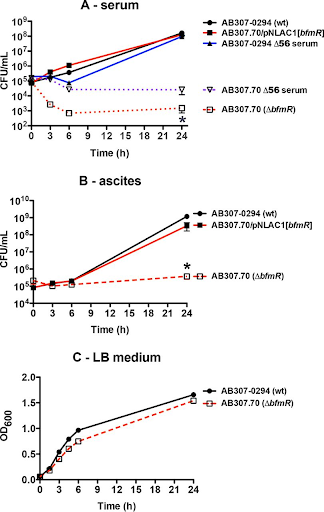
\includegraphics[scale=0.7]{survival-curve.png}
\caption{Survival Curves of \emph{Acinetobacter baumannii} \cite{beanan}}
\label{fig:survival-curve-a-baumannii}
\end{figure}

\begin{figure}[htbp]
\centering
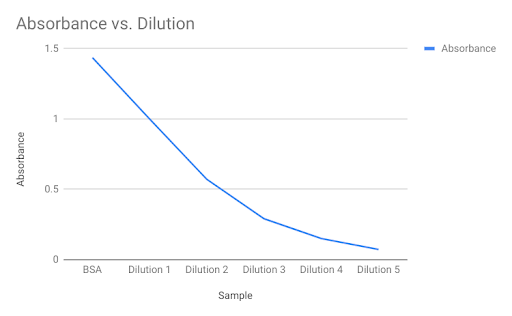
\includegraphics[scale=0.65]{bsa-dilution-curve.png}
\caption{Standard curve for BSA Dilution}
\label{fig:dilution-curve}
\end{figure}


\begin{figure}[htbp]
\centering
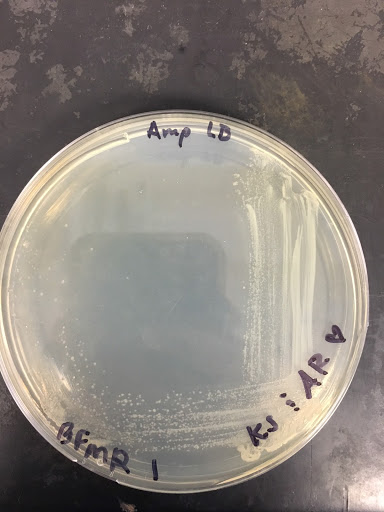
\includegraphics[scale=0.5]{streaked-bacteria.jpg}
\caption{Streaked Wild Type \emph{Acinetobacter baumannii}}
\label{fig:streaked-bacteria}
\end{figure}


\begin{figure}[htbp]
\centering
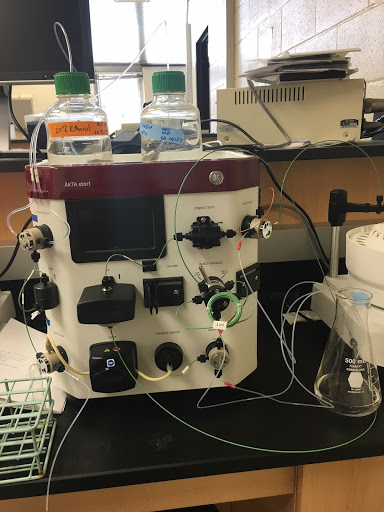
\includegraphics[scale=0.5]{chromatographic-machinery.jpg}
\caption{Fast Protein Liquid Chromatography Machinery to Purify BfmR Protein}
\label{fig:chromatography-machinery}
\end{figure}

\begin{figure}[htbp]
\centering
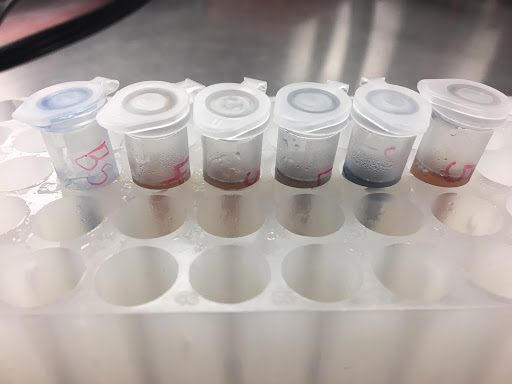
\includegraphics[scale=0.5]{dilution-bsa.jpg}
\caption{Bradford Dye Assay Dilution of BSA}
\label{fig:dilution-bsa}
\end{figure}

\begin{figure}[htbp]
\centering
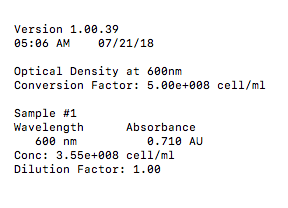
\includegraphics[scale=1.0]{OD-600nm.png}
\caption{OD 600 nm of \emph{A. baumannii}}
\label{fig:OD-600nm}
\end{figure}

\begin{figure}[htbp]
\centering
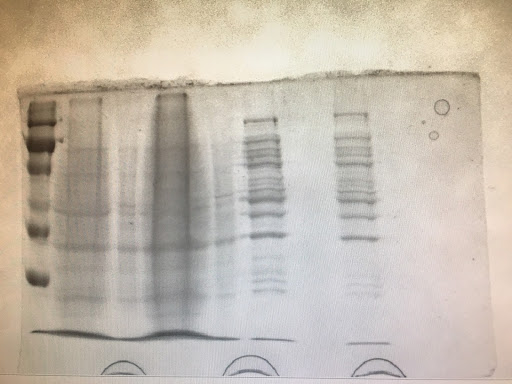
\includegraphics[scale=0.5]{sds-page-results.jpg}
\caption{SDS Page results of BfmR Protein}
\label{fig:sds-page-results}
\end{figure}


\begin{figure}[htbp]
\centering
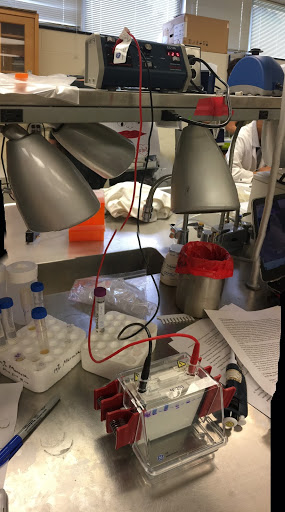
\includegraphics[scale=1.0]{sds-page-setup.jpg}
\caption{SDS Page Set Up}
\label{fig:sds-page-setup}
\end{figure}

\end{document}
